\documentclass[sigconf]{acmart}

\usepackage{booktabs} % For formal tables


% Copyright
%\setcopyright{none}
%\setcopyright{acmcopyright}
%\setcopyright{acmlicensed}
\setcopyright{rightsretained}
%\setcopyright{usgov}
%\setcopyright{usgovmixed}
%\setcopyright{cagov}
%\setcopyright{cagovmixed}


% DOI
\acmDOI{10.475/123_4}

% ISBN
\acmISBN{123-4567-24-567/08/06}

%Conference
\acmConference[WOODSTOCK'97]{ACM Woodstock conference}{July 1997}{El
  Paso, Texas USA}
\acmYear{1997}
\copyrightyear{2016}

\acmPrice{15.00}


\begin{document}
\title{Robotic cloth manipulation for clothing assistance task using Dynamic Movement
Primitives}
\titlenote{Produces the permission block, and copyright information}
%\subtitle{Extended Abstract}
%\subtitlenote{The full version of the author's guide is available as
%  \texttt{acmart.pdf} document}


\author{Ravi P. Joshi}
\authornote{Dr.~Trovato insisted his name be first.}
\orcid{1234-5678-9012}
\affiliation{%
	\institution{Institute for Clarity in Documentation}
	\streetaddress{P.O. Box 1212}
	\city{Dublin}
	\state{Ohio}
	\postcode{43017-6221}
}
\email{joshi-ravi-prakash@edu.brain.kyutech.ac.jp}

\author{Nishanth Koganti}
\authornote{The secretary disavows any knowledge of this author's actions.}
\affiliation{%
	\institution{Institute for Clarity in Documentation}
	\streetaddress{P.O. Box 1212}
	\city{Dublin}
	\state{Ohio}
	\postcode{43017-6221}
}
\email{nishanth-k@is.naist.jp}

\author{Tomohiro Shibata}
\authornote{This author is the
one who did all the really hard work.}
\affiliation{%
	\institution{The Th{\o}rv{\"a}ld Group}
	\streetaddress{1 Th{\o}rv{\"a}ld Circle}
	\city{Hekla}
	\country{Iceland}}
\email{tom@brain.kyutech.ac.jp}

%\author{Lawrence P. Leipuner}
%\affiliation{
%  \institution{Brookhaven Laboratories}
%  \streetaddress{P.O. Box 5000}}
%\email{lleipuner@researchlabs.org}
%
%\author{Sean Fogarty}
%\affiliation{%
%  \institution{NASA Ames Research Center}
%  \city{Moffett Field}
%  \state{California}
%  \postcode{94035}}
%\email{fogartys@amesres.org}
%
%\author{Charles Palmer}
%\affiliation{%
%  \institution{Palmer Research Laboratories}
%  \streetaddress{8600 Datapoint Drive}
%  \city{San Antonio}
%  \state{Texas}
%  \postcode{78229}}
%\email{cpalmer@prl.com}
%
%\author{John Smith}
%\affiliation{\institution{The Th{\o}rv{\"a}ld Group}}
%\email{jsmith@affiliation.org}
%
%\author{Julius P.~Kumquat}
%\affiliation{\institution{The Kumquat Consortium}}
%\email{jpkumquat@consortium.net}
%
% The default list of authors is too long for headers}
%\renewcommand{\shortauthors}{B. Trovato et al.}

\graphicspath{{./images/}}

\begin{abstract}
	The need of robotic clothing assistance in the field of assistive robotics is growing, as it is one of the most basic activities in daily life of elderly and disabled people. In this study, we are investigating the applicability of using Dynamic Movement Primitives (DMP) as a task parameterization model for performing clothing assistance tasks. The robotic cloth manipulation task deals with putting the cloth on both the arms. The robot should do cooperative manipulation by holding the cloth. Also, there can be many failure scenarios as clothes are highly non-rigid. DMP can represent nonlinear motion with a set of differential equations. These equations can be adapted to generate any movement trajectory just by changing the goal parameter. The system consists of Baxter humanoid robot and Microsoft Kinect RGBD sensor for tracking the posture of hands. To perform the task, a demonstration is recorded by moving the Baxter arms in the appropriate trajectory. The recorded trajectory is parameterized by using DMP. Once the system is trained, new postures are accommodated by DMP. The cloth manipulation is done by Baxter humanoid robot which follows the trajectory generated by DMP. We have performed the experiments on soft mannequin instead of human. The result shows that DMPs are able to generalize the movement trajectory for the modified posture also.
\end{abstract}

%
% The code below should be generated by the tool at
% http://dl.acm.org/ccs.cfm
% Please copy and paste the code instead of the example below.
%
\begin{CCSXML}
	<ccs2012>
	<concept>
	<concept_id>10010520.10010553.10010562</concept_id>
	<concept_desc>Computer systems organization~Embedded systems</concept_desc>
	<concept_significance>500</concept_significance>
	</concept>
	<concept>
	<concept_id>10010520.10010575.10010755</concept_id>
	<concept_desc>Computer systems organization~Redundancy</concept_desc>
	<concept_significance>300</concept_significance>
	</concept>
	<concept>
	<concept_id>10010520.10010553.10010554</concept_id>
	<concept_desc>Computer systems organization~Robotics</concept_desc>
	<concept_significance>100</concept_significance>
	</concept>
	<concept>
	<concept_id>10003033.10003083.10003095</concept_id>
	<concept_desc>Networks~Network reliability</concept_desc>
	<concept_significance>100</concept_significance>
	</concept>
	</ccs2012>
\end{CCSXML}

\ccsdesc[500]{Computer systems organization~Embedded systems}
\ccsdesc[300]{Computer systems organization~Redundancy}
\ccsdesc{Computer systems organization~Robotics}
\ccsdesc[100]{Networks~Network reliability}

% We no longer use \terms command
%\terms{Theory}

\keywords{Robotic Clothing Assistance, Dynamic Movement Primitives (DMP)}


\maketitle

\section{Introduction}

The \textit{proceedings} are the records of a conference\footnote{This
is a footnote}.  ACM seeks
to give these conference by-products a uniform, high-quality
appearance.  To do this, ACM has some rigid requirements for the
format of the proceedings documents: there is a specified format
(balanced double columns), a specified set of fonts (Arial or
Helvetica and Times Roman) in certain specified sizes, a specified
live area, centered on the page, specified size of margins, specified
column width and gutter size.

\section{Related Works}
Typically, the body of a paper is organized into a hierarchical
structure, with numbered or unnumbered headings for sections,
subsections, sub-subsections, and even smaller sections.  The command
\texttt{{\char'134}section} that precedes this paragraph is part of
such a hierarchy.\footnote{This is a footnote.} \LaTeX\ handles the
numbering and placement of these headings for you, when you use the
appropriate heading commands around the titles of the headings.  If
you want a sub-subsection or smaller part to be unnumbered in your
output, simply append an asterisk to the command name.  Examples of
both numbered and unnumbered headings will appear throughout the
balance of this sample document.

\section{Dynamic Movement Primitives}
Dynamic Movement Primitives (DMP) aims at designing contoller for learning and generalization of Motor Skills by learning from demonstration \cite{ijspeert2013dynamical}. The controllers are based on nonlinear dynamical systems, and use locally weighted regression techniques to learn complex, discrete or rhythmic, movements demonstrated by a human subject. These controllers can be considered to be discrete or rhythmic pattern generators which can replay and modulate the learned movements, while being robust against perturbations. 

The basic idea behind DMP formulation is to use an analytically well-understood dynamical system and add a nonlinear terms, so that it produces the desired behavior \cite{ijspeert2013dynamical}. Formally, the system is defined by a damped spring model as below:

\begin{equation}
	\ddot{y} = \alpha_y ( \beta_y (g - y) - \dot{y}) + f
\end{equation}

The term $\alpha_y$ and $\beta_y$ are positive gain terms. $y$ is the system state and $g$ represents goal state. The nonlinear function $f$, which is also called as forcing term is defined over time, making the problem a well defined structure that can be solved in a straight-forward way. This system is termed as canonical dynamical system, denoted by $x$ and has very simple dynamics:

\begin{equation}
	\dot{x} = -\alpha_x x
\end{equation}

The forcing function $f$ is chosen as a function of canonical system:

\begin{equation}
	f(x,g) = \frac{\Sigma_{i=1}^N \psi_i w_i}{\Sigma_{i=1}^N \psi_i} x(g - y_0)
	\label{forcing_func}
\end{equation}

with $N$ exponential basis functions $\psi_i$ and $y_0$ is the initial position of the system,

\begin{equation}
	\psi_i = \textrm{exp}\left( -h_i \left( x - c_i\right)^2 \right)
\end{equation}

where $h_i$ and $c_i$ are constants that determine, respectively, the width and centers of the basis functions. In this way, the forcing function $f$ is comprised of weighted summation of Gaussians, that are going to be activated as system converges to the goal as shown in figure \ref{psi_activations}.

\begin{figure}
	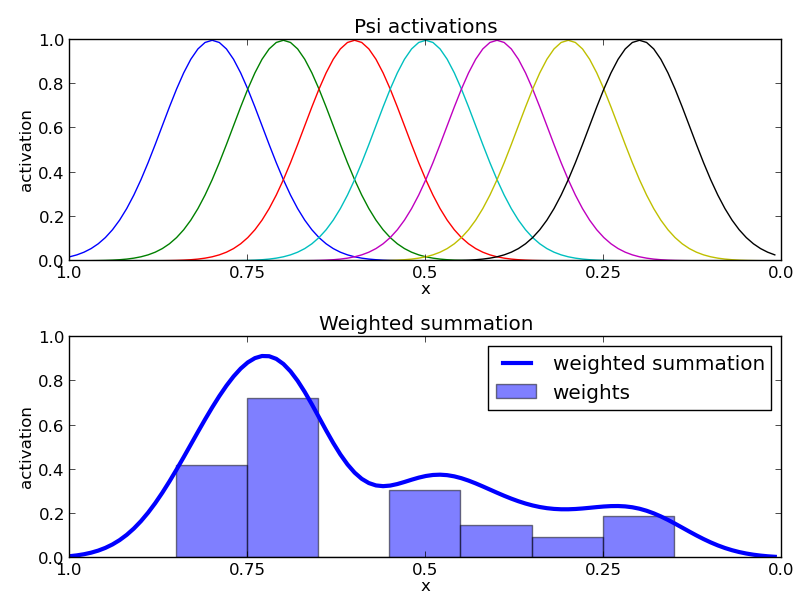
\includegraphics[width=0.45\textwidth]{psi}
	\caption{$\psi$ activations and weighted summation of Gaussians}
	\label{psi_activations}
\end{figure}

Our goal is to design the forcing function that can learn from the demonstration and allows us to scale the movement defined by goal state $g$. In other words, we want to setup the system which can follow a specified path. The forcing term can be redefined as:

\begin{equation}
	\textbf{f}_d = \ddot{\textbf{y}}_d - \alpha_y ( \beta_y (g - \textbf{y}) - \dot{\textbf{y}})
\end{equation}

where desired acceleration $\ddot{\textbf{y}}_d$ can be calculated by double differentiating the position data as:

\begin{equation*}
	\ddot{\textbf{y}}_d = \frac{\partial}{\partial t} \dot{\textbf{y}}_d = \frac{\partial}{\partial t} \frac{\partial}{\partial t} \textbf{y}_d
\end{equation*}

This ends by calculating the weight parameters across Gaussians. Optimization methods such as locally weighted regression can be used, so that the forcing function matches the desired trajectory. In other words equation can be re-written as-

\begin{equation}
	\Sigma_t \psi_i(t)(f_d(t) - w_i (x(t) (g - y_0)))^2
\end{equation}

The solution\cite{vijayakumar2000locally} is given by:

\begin{equation}
	w_i = \frac{\textbf{s}^T \pmb{\psi}_i \textbf{f}_d}{\textbf{s}^T \pmb{\psi}_i \textbf{s}}
\end{equation}

where
\begin{equation*}
	\textbf{s} = \left( \begin{array}{c}x_{t_0}(g - y_0) \\ \vdots \\ x_{t_N}(g - y_0) \end{array} \right), \;\;\; \pmb{\psi}_i = \left( \begin{array}{ccc} \psi_i(t_0) & \dots & 0 \\ 0 & \ddots & 0 \\ 0 & \dots & \psi_i(t_n) \end{array} \right)
\end{equation*}

This way the DMP can be made to imitate the desired path.

\section{Overview of the System}
Robotic cloth manipulation task contains a dual arm humanoid robot Baxter. The complete setup is shown in figure \ref{setup}. We choose soft mannequin instead of a human for this preliminary experiment. Both the arms of mannequin are open and  given the support by a metallic stand, to avoid falling down the arms. The mannequin is positioned in such a way, so that it resides within the limits of work space of the Baxter robot. Also both the arms of mannequin are facing towards robot. A kinect v2 sensor is mounted on the LCD display of Baxter root. Kinect sensor can see the mannequin and clothing article. Before starting the experiment, the clothing article is put in arms of the baxter robot manually.

\begin{figure}
	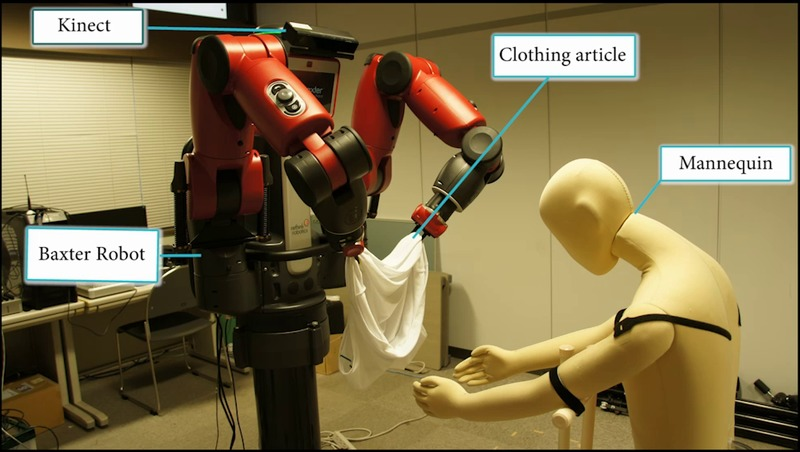
\includegraphics[width=0.45\textwidth]{setup}
	\caption{Setup of Robotic cloth manipulation task}
	\label{setup}
\end{figure}

The Baxter robot is connected to a computer directly using Ethernet cable. It is controlled using Robot Operating System (ROS), one of the widely used tool by the researchers in robotics community. We used Baxter robot's API, which are available and supported by ROS \cite{fitzgerald2013developing} to command the robot. The Kinect sensor is also controlled by Open source Kinect API for ROS.

\begin{figure*}
	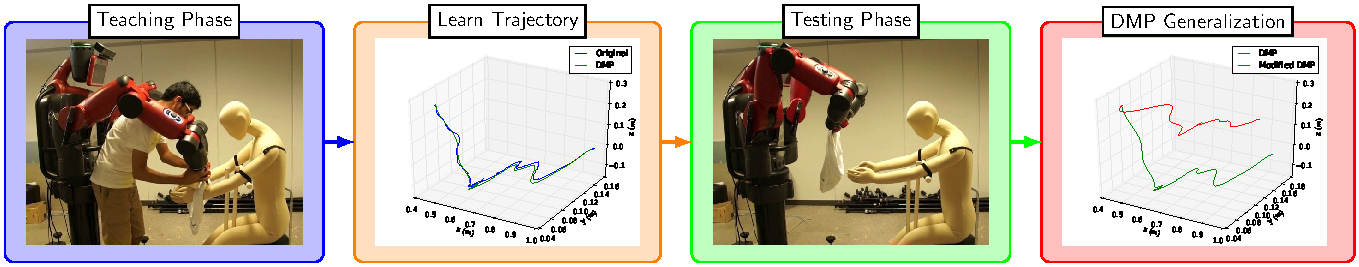
\includegraphics[width=\textwidth]{flowchart_conf}
	\caption{Work flow of Robotic cloth manipulation task. Initially a demonstration is performed by moving the Baxter arms in the appropriate trajectory. The demonstration is recorded and parameterized by DMP. Later posture of the mannequin is changed and accordingly the goal posture of DMP is modified. Now, the modified DMP can accommodate new posture.}
	\label{workflow}
\end{figure*}

\section{Experiments}
As per the formulation \ref{setup}, the DMP can learn by the demonstration. Hence we starts by performing a demonstration by holding the robot arm and move accordingly. During the demonstration, pose of the end-effector is recorded. The term pose collectively refers to position and orientation. Once the demonstration is finished, DMP is initialized using the recorded trajectory. Three DMP trajectories one for each coordinate axis are initialized for one arm. In this way, we have totally six DMP trajectories, which can control both the arms of Baxter robot. We performed following two experiments by using these trajectory- (a) Clothing task using position DMP (b) Failure detection using end-effector forces.

\subsection{Clothing task using position DMP}
The aim of this experiment is to put the clothing article on both the arms of mannequin by using DMP system. We use the position data to initialize the DMP trajectories, which are being used in this task. The posture of mannequin is changed by lifting the arms up or down. At this point, we use Kinect Sensor to get the 3D coordinates of the arm. Now we change the goal of DMP trajectories by using this information. The modified DMP can be acquired from equation 1.

\subsection{Failure detection using end-effector forces}
This experiment is designed to deal with failure cases. There can be many failure cases during the clothing task, such as the clothing article gets stuck into the fingers. In this experiment, we are using forces being applied on the end-effector of Baxter robot to detect the failure scenario. Appropriate action can be taken once the failure is detected.

\section{Results}
This paragraph will end the body of this sample document.
Remember that you might still have Acknowledgments or
Appendices; brief samples of these
follow.  There is still the Bibliography to deal with; and
we will make a disclaimer about that here: with the exception
of the reference to the \LaTeX\ book, the citations in
this paper are to articles which have nothing to
do with the present subject and are used as
examples only.

\section{Conclusions}
This paragraph will end the body of this sample document.
Remember that you might still have Acknowledgments or
Appendices; brief samples of these
follow.  There is still the Bibliography to deal with; and
we will make a disclaimer about that here: with the exception
of the reference to the \LaTeX\ book, the citations in
this paper are to articles which have nothing to
do with the present subject and are used as
examples only.

\begin{acks}
	The authors would like to thank Dr. Yuhua Li for providing the
	matlab code of  the \textit{BEPS} method. 
	
	The authors would also like to thank the anonymous referees for
	their valuable comments and helpful suggestions. The work is
	supported by the \grantsponsor{GS501100001809}{National Natural
		Science Foundation of
		China}{http://dx.doi.org/10.13039/501100001809} under Grant
	No.:~\grantnum{GS501100001809}{61273304}
	and~\grantnum[http://www.nnsf.cn/youngscientsts]{GS501100001809}{Young
	Scientsts' Support Program}.
	
\end{acks}

\bibliographystyle{ACM-Reference-Format}
\bibliography{sigproc}

\end{document}
